\documentclass[12pt,a4paper]{report}  
\usepackage{graphicx}
\usepackage{longtable}
\usepackage{float}% Required for inserting images
\usepackage{fancyhdr} % Required for header and footer
\usepackage{titlesec}
\usepackage{times}
\usepackage{listings}
\usepackage{xcolor}

\lstdefinestyle{phpstyle}{
  language=PHP,
  basicstyle=\ttfamily\small,
  keywordstyle=\color{blue},
  commentstyle=\color{gray},
  stringstyle=\color{red},
  tabsize=2,
  showspaces=false,
  showstringspaces=false,
  breaklines=true,
  numbers=none
}

\usepackage{geometry} 
\geometry{margin=1in}
\usepackage{setspace} 
\usepackage[backend=biber,style=numeric]{biblatex}
\addbibresource{references.bib} 
\setcounter{secnumdepth}{4}  
\setcounter{tocdepth}{4}  

\titleformat{\chapter}[hang]{\bfseries\Large}{\thechapter\ :}{1em}{}  

\titleformat{\chapter}
  {\vspace{-2cm} \centering\bfseries\LARGE} 
  {\thechapter}{1em}{}  

\begin{document}

\pagenumbering{roman}
\begin{titlepage}
    \centering
    \setstretch{1.5}
    
    {\fontsize{18pt}{22pt}\selectfont \textbf{RAJAGIRI COLLEGE OF SOCIAL SCIENCES}}\\[0.2cm]
    {\fontsize{16pt}{20pt}\selectfont \textbf{(AUTONOMOUS)}}\\[0.2cm]
    {\fontsize{16pt}{20pt}\selectfont \textbf{KALAMASSERY}}\\[1.5cm]
    
    [INSERT IMAGE HERE: Rajagiri College Logo]\\[1.5cm]
    
    {\fontsize{16pt}{20pt}\selectfont \textbf{Department of Computer Science}}\\[1cm]
    
    {\fontsize{18pt}{22pt}\selectfont \textbf{FSD Project Report}}\\[1cm]
    
    {\fontsize{20pt}{24pt}\selectfont \textbf{ParkX - Smart Parking Management System}}\\[2cm]
    
    {\fontsize{16pt}{20pt}\selectfont \textbf{Done by}}\\[0.2cm]
    {\fontsize{18pt}{22pt}\selectfont \textbf{Amal Biju}}\\[0.2cm]
    {\fontsize{16pt}{20pt}\selectfont \textbf{Reg No: 24118005}}\\[2cm]
    
    {\fontsize{16pt}{20pt}\selectfont \textbf{2024-2028}}
\end{titlepage}

\newpage
\begin{titlepage}
\begin{center}
    \setstretch{1.5}
    {\fontsize{18pt}{22pt}\selectfont \textbf{RAJAGIRI COLLEGE OF SOCIAL SCIENCES}}\\[0.2cm]
    {\fontsize{16pt}{20pt}\selectfont \textbf{(AUTONOMOUS)}}\\[0.2cm]
    {\fontsize{16pt}{20pt}\selectfont \textbf{KALAMASSERY}}\\[1cm]
    
    [INSERT IMAGE HERE: Rajagiri College Logo]\\[1cm]
    
    {\fontsize{18pt}{22pt}\selectfont \textbf{CERTIFICATE}}\\[1cm]
\end{center}

\noindent
This is to certify that the FSD Project Report entitled \textbf{"ParkX - Smart Parking Management System"} is a bona fide record of the work done by \textbf{Amal Biju} (Register No: \textbf{24118005}) under my supervision during the academic year 2024-2028.

\vfill

\noindent
\begin{minipage}[t]{0.5\textwidth}
\raggedright
\textbf{Project Coordinator} \\
Dr. Bindhiya M Varghese
\end{minipage}
\hfill
\begin{minipage}[t]{0.45\textwidth}
\raggedleft
\textbf{Faculty Guide} \\
Mr. Ajay Joseph Antony
\end{minipage}

\vspace{3cm}

\noindent
\begin{minipage}[t]{0.5\textwidth}
\raggedright
\textbf{External Examiner} \\
\rule{5cm}{0.4pt}
\end{minipage}
\hfill
\begin{minipage}[t]{0.45\textwidth}
\raggedleft
\textbf{Internal Examiner} \\
\rule{5cm}{0.4pt}
\end{minipage}
\end{titlepage}

\newpage
\setstretch{1.15} 

\setcounter{page}{1} % Set acknowledgement to roman i
\chapter*{ \begin{center} 
    \textbf{\LARGE ACKNOWLEDGEMENTS}  
\end{center} }  
\addcontentsline{toc}{chapter}{ACKNOWLEDGEMENT}  

I would like to express my sincere gratitude to all those who helped me in the successful completion of this project.

First and foremost, I would like to thank \textbf{[Your Faculty Name]} for their invaluable guidance, constant supervision, and encouragement throughout the course of this project. Their deep insights and continuous feedback helped shape ParkX into a robust and scalable application.

I am also deeply grateful to the Head of the Department, \textbf{[HOD Name]}, and the entire faculty of the Computer Science Department at Rajagiri College of Social Sciences, for providing the necessary facilities and an excellent learning environment. 

Finally, I would like to thank my family and friends for their continuous support and encouragement which helped me to stay focused and motivated during the development of this project.

\vspace{2cm}

\noindent \textbf{Amal Biju}

\newpage
\chapter*{ \begin{center} 
    \textbf{\LARGE ABSTRACT}  
\end{center} }  
\addcontentsline{toc}{chapter}{ABSTRACT}  
\vspace{-2cm}  
 

ParkX is an innovative Smart Parking Management System developed using the Laravel framework and modern frontend tools. It is designed to mitigate the growing challenges of urban parking, such as inefficient slot management, unorganized booking systems, and revenue leakage for parking owners. The platform serves as a multi-tier solution featuring three core modules: User, Owner, and Admin.

\\\\
The system allows ordinary Users to search and intuitively book parking slots across various venues, categorized dynamically based on vehicle type. An integrated "Antigravity" UI structure presents a premium experience for user interactions, from slot selection on a customized architectural map to seamless payment integration. Meanwhile, the Owner module empowers property administrators to list parking venues, manage slots, establish pricing strategies, and securely view bookings in real time. The Super Admin module operates as the overarching governance system, approving property registrations, monitoring system-wide analytics, and ensuring fluid communication between all network participants.

\\\\
Implementing robust Role-Based Access Control (RBAC) via Laravel Middleware and leveraging MySQL for structured data persistence, ParkX promises a modernized, accessible, and scalable architecture optimized for 21st-century mobility infrastructure.

\newpage

\renewcommand{\baselinestretch}{1.15}  
\selectfont  

\renewcommand{\contentsname}{\hfill \LARGE \textbf{CONTENTS} \hfill} 
\tableofcontents
\newpage

\addcontentsline{toc}{chapter}{LIST OF TABLES} 
\renewcommand{\listtablename}{\hfill \LARGE \textbf{LIST OF TABLES} \hfill} 
\listoftables
\newpage

\addcontentsline{toc}{chapter}{LIST OF FIGURES} 
\begin{center}
    \LARGE \textbf{LIST OF FIGURES}
\end{center}

\vspace{0.5cm}

\noindent
\begin{longtable}{p{2cm} p{10cm} r}
    \textbf{Figure No.} & \textbf{Title} & \textbf{Page No.} \\
    \hline
    \endhead
    Figure 4.1 & Use Case Diagram \dotfill & \pageref{fig:use_case} \\
    Figure 4.2 & Activity Diagram (User Booking Flow) \dotfill & \pageref{fig:activity} \\
    Figure 4.3 & System Architecture Diagram \dotfill & \pageref{fig:architecture} \\
    Figure 4.4 & Class Diagram \dotfill & \pageref{fig:class} \\
    Figure 4.5 & Entity-Relationship (ER) Diagram \dotfill & \pageref{fig:er} \\
    Figure 4.6 & Sequence Diagram (Transactional Slot Locking) \dotfill & \pageref{fig:sequence} \\
    Figure 4.7 & Project Pipeline \dotfill & \pageref{fig:pipeline} \\
    Figure 7.1 & Git Commit History \dotfill & \pageref{fig:git} \\
\end{longtable}

\newpage
\pagestyle{fancy}
\fancyhf{}  
\fancyhead[R]{{ParkX - Smart Parking System}}

\renewcommand{\footrulewidth}{0.4pt} 
\fancyfoot[L]{Department of Computer Science, RCSS} 
\fancyfoot[R]{\thepage} 

\fancypagestyle{plain}{%
  \fancyhf{}
  \fancyhead[R]{{ParkX - Smart Parking System}}
  \renewcommand{\footrulewidth}{0.4pt} 
  \fancyfoot[L]{Department of Computer Science, RCSS}
  \fancyfoot[R]{\thepage}
}

\fancypagestyle{noheaderfooter}{
    \fancyhf{} 
    \renewcommand{\headrulewidth}{0pt} 
    \renewcommand{\footrulewidth}{0pt} 
}
\pagenumbering{arabic}

\chapter{INTRODUCTION}

\section{Overview}
The rapid pace of global urbanization has exerted significant pressure on city infrastructure, with vehicle parking emerging as one of the most critical challenges. In densely populated urban centers, the perennial struggle to find available parking leads to increased fuel consumption, elevated carbon emissions, and substantial productivity losses. Traditional manual parking management systems are often inefficient, lack real-time visibility, and fail to provide the seamless experience expected in the digital age.

\textbf{ParkX} is a sophisticated, centralized Smart Parking Management System engineered to address these challenges through digital innovation. Developed as a comprehensive solo project by \textbf{Amal Biju}, ParkX leverages the robust \textbf{Laravel PHP Framework}, \textbf{PostgreSQL}, and the \textbf{Tailwind CSS CDN} to provide a high-performance, aesthetically premium platform connecting parking space owners with vehicle drivers. By providing real-time slot visibility and advanced booking capabilities, the system optimizes space utilization and significantly enhances user convenience.

\section{Objectives}
The primary objectives of the ParkX Smart Parking Management System are:
\begin{itemize}
    \item \textbf{Intelligent Discovery and Reservation:} To empower drivers with a visual interface for locating, reviewing, and instantly reserving parking slots in real-time.
    \item \textbf{Dynamic Resource Management:} To provide parking lot owners with a dedicated portal for listing venues and categorized slots (e.g., Two-Wheeler, Four-Wheeler) while monitoring occupancy metrics.
    \item \textbf{Centralized Platform Governance:} To establish a Super Admin dashboard for comprehensive oversight, including owner approval, system-wide taxonomy management, and activity auditing.
    \item \textbf{Premium User Experience:} To implement a modern "Antigravity" design language featuring glassmorphism and smooth micro-interactions to ensure high engagement and accessibility.
\end{itemize}

\section{Scope of the Project}
The ParkX system is initially implemented as a localized web-based platform capable of managing concurrent users and secure transactions. It incorporates a sophisticated Role-Based Access Control (RBAC) architecture that strictly segregates Administrative, Ownership, and User functionalities. 

A key focus of this release is the implementation of a \textbf{Manual Ticket PIN Fallback} system, ensuring that check-ins can be processed securely via a unique 6-digit alphanumeric code even when QR scanners are unavailable. While the current version emphasizes slot visualization and manual check-in verification, the modular architecture is designed for future scaling, including integration with IoT sensors, automated barriers, and direct payment gateway APIs.

\chapter{SUPPORTING LITERATURE}

\section{Existing Systems}
Traditionally, parking management relied on manual ticketing, cash-based payments, and physical guards directing vehicles to vacant slots. These systems presented numerous flaws:
\begin{itemize}
    \item \textbf{High Wait Times:} Manual ticket generation slows down entry processes during peak hours, causing long queues on major roads.
    \item \textbf{Lack of Real-time Data:} Drivers circle blocks aimlessly because there is no prior knowledge of slot availability.
    \item \textbf{Revenue Leakages:} Manual accounting significantly increases the chance of unrecorded transactions or human error, penalizing the property owner.
    \item \textbf{Suboptimal Utilization:} Large properties often have segmented lots where distant slots remain empty simply because drivers are unaware of them.
\end{itemize}

\section{Transition to Smart Solutions}
Recent years have seen the implementation of semi-automated models, primarily using RFID cards or boom barriers. However, these systems often lack a user-facing booking interface that allows discovery *prior* to arrival. Mobile applications exist, but they are often highly fragmented, requiring drivers to download different apps for different parking providers.

\section{The ParkX Approach}
ParkX improves upon the current literature and existing deployments by acting as an aggregator. Rather than belonging to a single parking complex, ParkX operates as a multi-tenant platform. Property owners register their venues on the platform, and the Super Admin vets and approves them. Once approved, all users on the ParkX network can discover and book slots at those venues. 

This approach minimizes fragmentation, centralizes the software architecture, and applies a modern tech stack (Laravel 12, Tailwind CSS \cite{tailwindcss}, Alpine.js \cite{alpinejs}) to ensure the platform feels fast, secure \cite{laravel_docs}, and responsive across all devices.

\chapter{SYSTEM ANALYSIS}

\section{Module Description}
The ParkX application is architected into three primary horizontal modules, each optimized for specific stakeholder workflows:

\begin{itemize}
    \item \textbf{User Module:} Provides drivers with an intuitive interface for discovering parking venues and reserving specific slots. Features include secure authentication, category-based slot filtering, architectural grid visualization for slot selection, and a personal booking history dashboard.
    \item \textbf{Owner Module:} Designed for parking facility managers. Owners can register and, upon administrative approval, manage their parking assets. This includes adding/editing parking spaces, defining individual slots, categorizing them by vehicle type, and monitoring live check-ins through both QR scanning and manual PIN verification.
    \item \textbf{Admin Module:} The governing layer of the platform. The Super Admin monitors platform-wide analytics, manages the global taxonomy of vehicle categories, and audits user/owner activity to ensure platform integrity.
\end{itemize}

\section{Business Rules}
The operational logic of ParkX is governed by strict business rules to ensure transactional safety and resource optimization.

\textbf{Authentication and Role Segregation}
\begin{itemize}
    \item All core system interactions require valid authentication.
    \item Role-Based Access Control (RBAC) enforces strict boundary management; Administrative settings are inaccessible to Owners, and Ownership tools are inaccessible to standard Users.
\end{itemize}

\textbf{Booking and Transactional Integrity}
\begin{itemize}
    \item \textbf{Conflict Resolution:} No single slot can be reserved for overlapping time windows. The backend employs PostgreSQL row-level locking (\textbf{FOR UPDATE}) to prevent race conditions during concurrent booking attempts.
    \item \textbf{Category Matching:} Slots must be associated with a predefined Vehicle Category. Drivers are required to select their vehicle type upfront, ensuring they are only presented with compatible parking options.
    \item \textbf{Check-in Validation:} Arrival at a venue is verified via QR code scanning. A mandatory 15-minute buffer is enforced for early arrivals, and expired tickets are automatically rejected.
    \item \textbf{Manual Fallback:} In scenarios where QR scanning is technically unfeasible, the system provides a manual check-in mechanism using a unique, 6-digit alphanumeric Ticket PIN.
\end{itemize}

\section{Use Case Model}
The Use Case Model identifies the foundational interactions between stakeholders and the system.

\subsection{Use Case Descriptions}
The following table summarizes the key automated events within the project lifecycle:

\begin{longtable}{|p{2cm}|p{4cm}|p{8cm}|}
    \caption{Foundational Use Cases} \label{tab:use_cases} \\
    \hline
    \textbf{ID} & \textbf{Use Case} & \textbf{Description} \\
    \hline
    \endfirsthead
    \hline
    \textbf{ID} & \textbf{Use Case} & \textbf{Description} \\
    \hline
    \endhead
    UC01 & Authentication & User/Owner authenticates securely with the platform. \\
    \hline
    UC02 & Venue Management & Owners create and configure physical parking spaces and slots. \\
    \hline
    UC03 & Slot Reservation & Users filter by category and reserve slots in real-time. \\
    \hline
    UC04 & Check-in / Manual PIN & System validates arrival via QR or 6-digit backup PIN. \\
    \hline
    UC05 & Analytics & Super Admin monitors global utilization and manages taxonomy. \\
    \hline
\end{longtable}

\section{System Architecture}
\subsection{Logical Framework}
The backend relies on the \textbf{Laravel PHP Framework}, utilizing an MVC (Model-View-Controller) architecture to separate data structures, business logic, and presentation layers. Data integrity is maintained through \textbf{PostgreSQL}, chosen for its robust support for complex transactions and ACID compliance.

The frontend is built using the \textbf{Tailwind CSS CDN}, ensuring a responsive, high-performance interface with a minimalist design language focused on "Antigravity" aesthetics.

\section{Feasibility Analysis}

\subsection{Technical Feasibility}
The project leverages the industry-standard Laravel framework and PostgreSQL database, providing a scalable and secure foundation. Technical risks are mitigated by utilizing native Laravel security features (XSS/CSRF protection) and PostgreSQL's explicit row-level locking for atomic booking resolution. The use of a CDN for Tailwind CSS ensures that the application remains lightweight without requiring complex build pipelines.

\subsection{Economical Feasibility}
ParkX is highly cost-effective as it is built entirely using open-source technologies. By utilizing the Laravel framework, PostgreSQL, and Composer-based dependency management, the project incurs zero licensing overhead for development or basic deployment.

\subsection{Operational Feasibility}
The system modernizes traditional parking workflows by replacing manual logs with a centralized digital dashboard. The inclusion of a manual fallback PIN ensures high operational reliability, allowing owners to maintain service even during scanner failures. The interface is designed for minimal learning curves, featuring visual slot status indicators.

\section{System Environment}

\subsection{Hardware Environment}
\begin{itemize}
    \item \textbf{Processor:} i5 10th Gen or equivalent (Recommended)
    \item \textbf{Memory:} 8 GB RAM
    \item \textbf{Storage:} 500 MB for core application and logs.
    \item \textbf{OS:} Windows 11 / Linux
\end{itemize}

\subsection{Software Environment}
\begin{itemize}
    \item \textbf{Runtime:} PHP 8.2+
    \item \textbf{Framework:} Laravel 12
    \item \textbf{Database:} PostgreSQL
    \item \textbf{Styling:} Tailwind CSS (via CDN)
    \item \textbf{Server:} Apache (via XAMPP for local development)
\end{itemize}

\section{Actors and Roles}

\textbf{Actor: User}\\
\textbf{Role:} Browses available venues, filters by category, reserves slots, and monitors personal booking history.

\textbf{Actor: Property Owner}\\
\textbf{Role:} Lists parking venues, defines slot geometry, and manages vehicle arrivals via QR/PIN verification.

\textbf{Actor: Super Admin}\\
\textbf{Role:} Governs the platform, approves owner registrations, and manages the global taxonomy of vehicle categories.

\chapter{SYSTEM DESIGN}

\section{Project Design}
System design is the process of defining the architecture, components, modules, interfaces, and data for a system to satisfy specified requirements. In ParkX, the design architecture is built around an MVC (Model-View-Controller) structure, specifically customized to support high-concurrency parking operations with atomic transactional hold times.

\subsection{Consolidated System Diagrams}
As per the project requirements, all foundational architectural and logical diagrams are consolidated below to provide a unified overview of the system's design.

\vspace{1cm}
\begin{figure}[H]
    \centering
    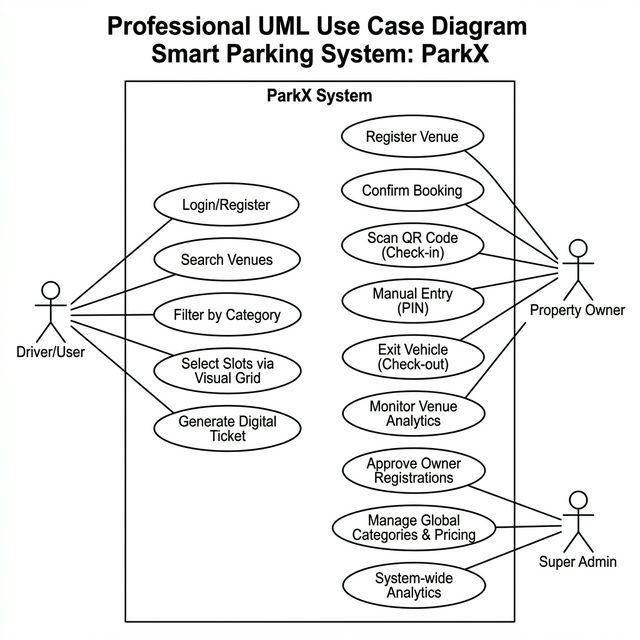
\includegraphics[width=0.9\textwidth]{diag_use_case.png}
    \caption{UML Use Case Diagram - System Boundary \& Actors}
    \label{fig:use_case}
\end{figure}
\vspace{1cm}

\vspace{1cm}
\begin{figure}[H]
    \centering
    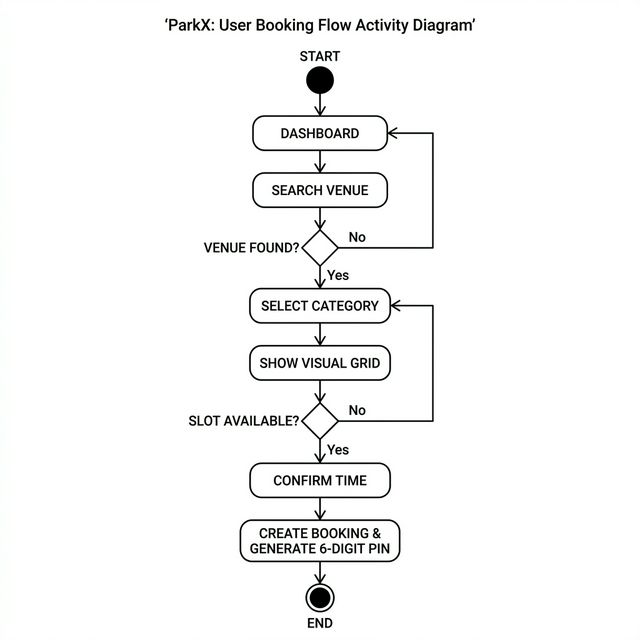
\includegraphics[width=0.9\textwidth]{diag_activity_booking.png}
    \caption{Activity Diagram - User Booking Flow}
    \label{fig:activity}
\end{figure}
\vspace{1cm}


\begin{figure}[H]
    \centering
    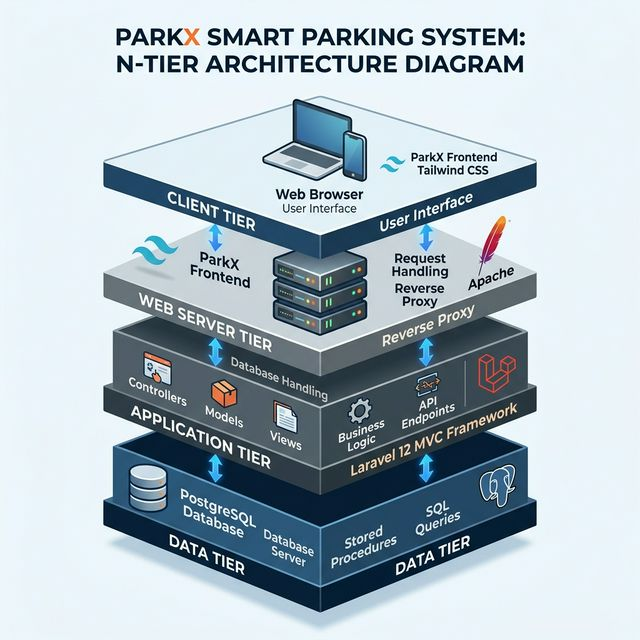
\includegraphics[width=0.9\textwidth]{diag_system_architecture.png}
    \caption{System Architecture Diagram}
    \label{fig:architecture}
\end{figure}
\vspace{1cm}

\vspace{1cm}
\begin{figure}[H]
    \centering
    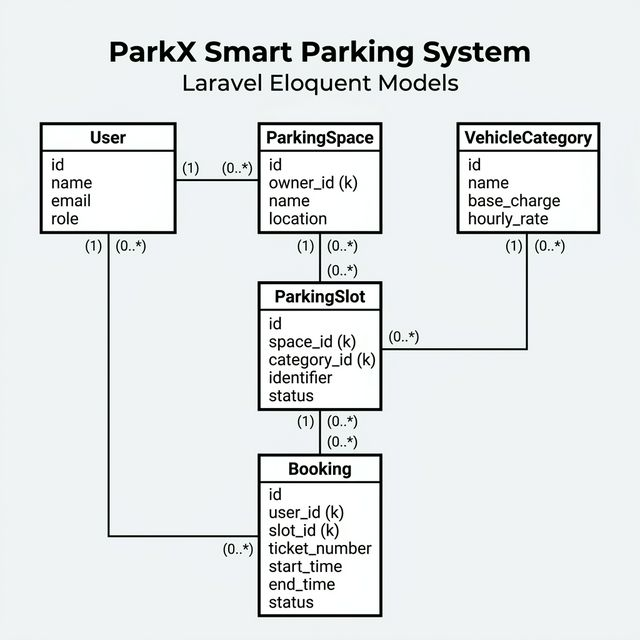
\includegraphics[width=0.9\textwidth]{diag_class_diagram_models.png}
    \caption{UML Class Diagram - Eloquent Models}
    \label{fig:class}
\end{figure}
\vspace{1cm}

\vspace{1cm}
\begin{figure}[H]
    \centering
    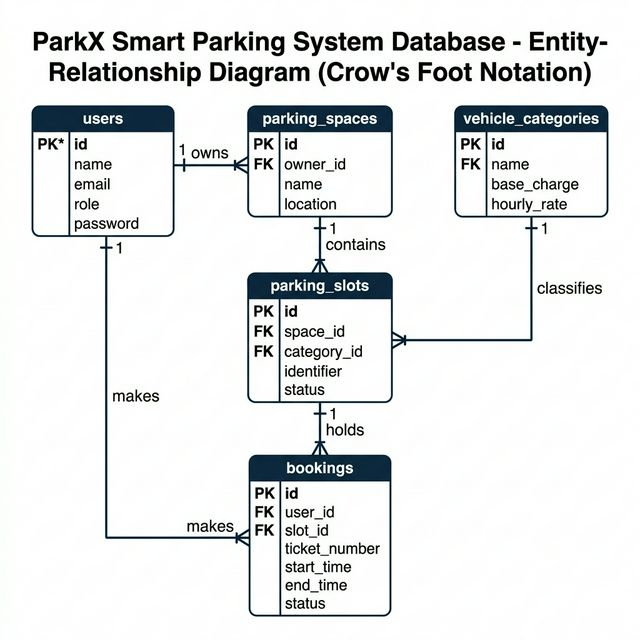
\includegraphics[width=0.9\textwidth]{diag_er_diagram_schema.png}
    \caption{Entity-Relationship (ER) Diagram}
    \label{fig:er}
\end{figure}
\vspace{1cm}

\vspace{1cm}
\begin{figure}[H]
    \centering
    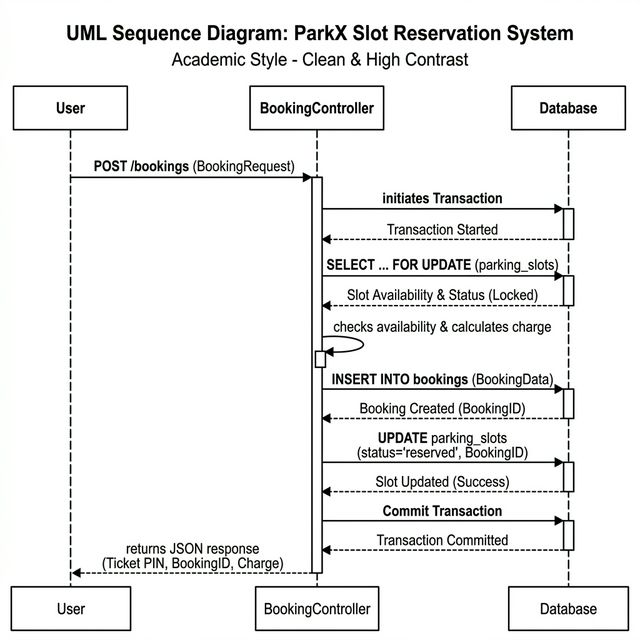
\includegraphics[width=0.9\textwidth]{diag_sequence_locking.png}
    \caption{Sequence Diagram (Transactional Slot Locking)}
    \label{fig:sequence}
\end{figure}
\vspace{1cm}

\begin{figure}[H]
    \centering
    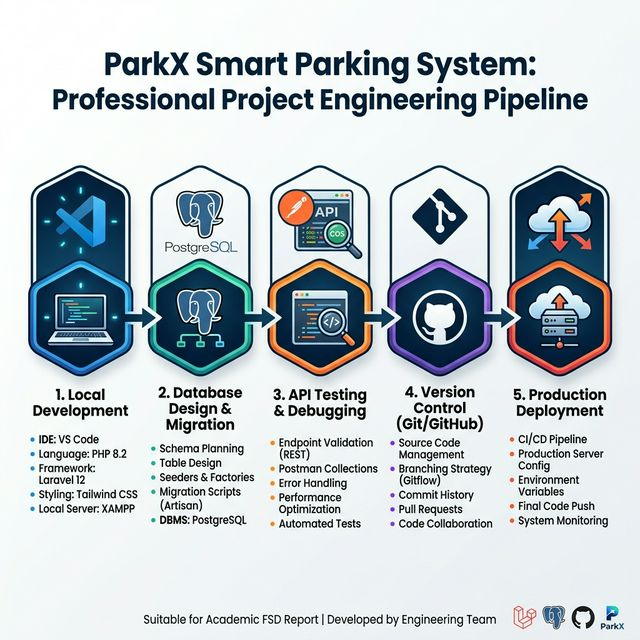
\includegraphics[width=0.9\textwidth]{diag_project_pipeline.png}
    \caption{Project Pipeline}
    \label{fig:pipeline}
\end{figure}
\vspace{1cm}

\section{User Interface (UI) Design}
The user interface of ParkX adheres to the "Antigravity" design blueprint, which emphasizes minimalism, depth, and smooth interactions.

\subsection{Design Aesthetics}
The interface utilizes semi-transparent glassmorphism elements, vibrant gradients, and high-contrast typography (Inter/Oswald) to create a premium, modern feel. Micro-interactions and subtle transitions are employed to provide immediate feedback to the driver or property owner.

\subsection{UI Review (Screenshots)}
The following represent the core interface screens of the ParkX application:

\vspace{0.5cm}
[INSERT IMAGE HERE: Figure 4.8 - Landing Page UI]
\vspace{0.5cm}

\vspace{0.5cm}
[INSERT IMAGE HERE: Figure 4.9 - Authentication Portal]
\vspace{0.5cm}

\vspace{0.5cm}
[INSERT IMAGE HERE: Figure 4.10 - Super Admin Dashboard]
\vspace{0.5cm}

\vspace{0.5cm}
[INSERT IMAGE HERE: Figure 4.11 - Owner Management Hub]
\vspace{0.5cm}

\vspace{0.5cm}
[INSERT IMAGE HERE: Figure 4.12 - User Booking Interface with Slot Grid]
\vspace{0.5cm}

\section{Database Design}
ParkX utilizes a highly normalized relational database implemented in \textbf{PostgreSQL}. The schema is designed to ensure referential integrity while supporting the high-concurrency needs of real-time slot selection.

\newpage
\subsection{Core Entity Tables}

\paragraph{Table: \textbf{users}}
Stores authentication, identification, and role-based credentials.
\begin{longtable}{|p{3cm}|p{3cm}|p{2cm}|p{6cm}|}
    \hline
    \textbf{Attribute} & \textbf{Data Type} & \textbf{Key} & \textbf{Description} \\
    \hline
    \endhead
    id & BigSerial & PK & Primary unique identifier \\
    \hline
    name & Varchar(255) & - & Full name of the user \\
    \hline
    email & Varchar(255) & Unique & Login email address \\
    \hline
    role & Varchar(20) & - & Roles: 'admin', 'owner', 'user' \\
    \hline
    password & Varchar(255) & - & Bcrypt hashed password \\
    \hline
\end{longtable}

\paragraph{Table: \textbf{vehicle\_categories}}
Maintains the global taxonomy of vehicle types and their associated pricing logic.
\begin{longtable}{|p{3cm}|p{3cm}|p{2cm}|p{6cm}|}
    \hline
    \textbf{Attribute} & \textbf{Data Type} & \textbf{Key} & \textbf{Description} \\
    \hline
    \endhead
    id & BigSerial & PK & Unique category ID \\
    \hline
    name & Varchar(255) & - & E.g., 'Two Wheeler' \\
    \hline
    base\_charge & Decimal(8,2) & - & Flat entry fee \\
    \hline
    hourly\_rate & Decimal(8,2) & - & Incremental cost per hour \\
    \hline
\end{longtable}

\subsection{Inventory and Infrastructure Tables}

\paragraph{Table: \textbf{parking\_spaces}}
Represents physical venues managed by owners.
\begin{longtable}{|p{3cm}|p{3cm}|p{2cm}|p{6cm}|}
    \hline
    \textbf{Attribute} & \textbf{Data Type} & \textbf{Key} & \textbf{Description} \\
    \hline
    \endhead
    id & BigSerial & PK & Unique venue ID \\
    \hline
    owner\_id & BigInt & FK & References \textbf{users.id} \\
    \hline
    name & Varchar(255) & - & Venue name \\
    \hline
    location & Text & - & Physical GIS/Address details \\
    \hline
\end{longtable}

\paragraph{Table: \textbf{parking\_slots}}
The atomic unit of inventory within a parking space.
\begin{longtable}{|p{3cm}|p{3cm}|p{2cm}|p{6cm}|}
    \hline
    \textbf{Attribute} & \textbf{Data Type} & \textbf{Key} & \textbf{Description} \\
    \hline
    \endhead
    id & BigSerial & PK & Unique slot ID \\
    \hline
    space\_id & BigInt & FK & References \textbf{parking\_spaces.id} \\
    \hline
    category\_id & BigInt & FK & References \textbf{vehicle\_categories.id} \\
    \hline
    identifier & Varchar(50) & - & E.g., 'A1', 'P-04' \\
    \hline
    status & Enum & - & 'available', 'occupied', 'reserved' \\
    \hline
\end{longtable}

\subsection{Transactional Tables}

\paragraph{Table: \textbf{bookings}}
Logs the orchestration between users and reserved slots.
\begin{longtable}{|p{3cm}|p{3cm}|p{2cm}|p{6cm}|}
    \hline
    \textbf{Attribute} & \textbf{Data Type} & \textbf{Key} & \textbf{Description} \\
    \hline
    \endhead
    id & BigSerial & PK & Unique booking ID \\
    \hline
    user\_id & BigInt & FK & References \textbf{users.id} \\
    \hline
    slot\_id & BigInt & FK & References \textbf{parking\_slots.id} \\
    \hline
    ticket\_number & Varchar(6) & Unique & Manual fallback PIN code \\
    \hline
    start\_time & Timestamp & - & Scheduled entry time \\
    \hline
    end\_time & Timestamp & - & Scheduled exit time \\
    \hline
    scanned\_at & Timestamp & - & Actual check-in timestamp \\
    \hline
    status & Varchar(20) & - & 'booked', 'occupied', 'completed' \\
    \hline
\end{longtable}

\chapter{TESTING}
Testing is a fundamental pillar of software reliability. In the context of the ParkX Smart Parking Management System, a wide array of test metrics were applied to ensure transactional safety, responsive cross-browser rendering, and strict role segregation.

\section{Unit Testing}
Unit testing ensures that individual database models, controllers, and validation rules operate correctly independent of the broader application structure.

\begin{longtable}{|p{1.5cm}|p{2.5cm}|p{4cm}|p{4cm}|c|}
    \hline
    \textbf{Test ID} & \textbf{Component} & \textbf{Test Description} & \textbf{Expected Result} & \textbf{Status} \\
    \hline
    \endfirsthead
    \hline
    \textbf{Test ID} & \textbf{Component} & \textbf{Test Description} & \textbf{Expected Result} & \textbf{Status} \\
    \hline
    \endhead
    \hline
    \endfoot
    \hline
    \caption{Unit Test Cases for ParkX} \label{tab:unit_tests} \\
    \endlastfoot

    UT01 & Login Logic & \raggedright Verify user authentication against bcrypt hashes & \raggedright Authentic users login; false passwords reject & Pass \\
    \hline
    UT02 & Middleware & \raggedright Access Owner dashboard as an standard User & \raggedright System blocks access and redirects & Pass \\
    \hline
    UT03 & Form Validation & \raggedright Submit booking form lacking a slot\_id selection & \raggedright Validation error prevents processing & Pass \\
    \hline
    UT04 & DB Creation & \raggedright Create slot via Owner controller & \raggedright Valid slot entry appears in DB via Eloquent & Pass \\
\end{longtable}

\section{Integration Testing}
Integration testing verifies that the interaction between diverse modules performs effectively, such as checking if user bookings effectively reduce available slot capacity metrics.

\begin{table}[H]
    \centering
    \renewcommand{\arraystretch}{1.3}
    \small
    \begin{tabular}{|c|p{3cm}|p{3cm}|p{3cm}|c|}
        \hline
        \textbf{Test ID} & \textbf{Component} & \textbf{Test Description} & \textbf{Expected Result} & \textbf{Status} \\
        \hline
        IT01 & Booking \& Slots & Valid user books an available Owner slot & Slot status associates correctly, booking confirms & Pass \\
        \hline
        IT02 & Category Sync & Admin deletes a Vehicle Category & Associated cascading/warning logic triggers safely & Pass \\
        \hline
        IT03 & UI Rendering & Alpine.js dynamic category filtering & Relevant slots populate upon category selection without page reload & Pass \\
        \hline
    \end{tabular}
    \caption{Integration Test Cases for ParkX}
    \label{tab:integration_tests}
\end{table}

\section{System Testing}
System testing evaluates the deployed application as an entire closed system via a browser, simulating accurate user flows.

\begin{table}[H]
    \centering
    \renewcommand{\arraystretch}{1.3}
    \begin{tabular}{|c|c|p{4cm}|p{3cm}|c|}
        \hline
        \textbf{Test ID} & \textbf{Component} & \textbf{Test Description} & \textbf{Expected Result} & \textbf{Status} \\
        \hline
        ST01 & Full App Launch & Verify local execution via \texttt{php artisan serve} & Application loads on designated PORT & Pass \\
        \hline
        ST02 & UI Responsiveness & Shrink screen to mimic mobile display & Tailwind CSS restructures grid to column layout & Pass \\
        \hline
        ST03 & Concurrency & Multiple users hit the booking endpoint simultaneously & InnoDB locks prevent double booking over shared slots & Pass \\
        \hline
    \end{tabular}
    \caption{System Test Cases for ParkX}
    \label{tab:system_tests}
\end{table}

\section{Security \& Performance Testing}
Performance and security testing validates that ParkX remains resilient against bad actors and resource exhaustion.

\begin{itemize}
    \item \textbf{CSRF Tokens:} All forms include \texttt{@csrf} directives, verified successfully by intercepting POST requests and observing 419 Page Expired errors on missing tokens.
    \item \textbf{Load Times:} Vite Hot-Module Replacement (HMR) combined with Laravel backend renders most view changes within 200ms latency locally.
\end{itemize}

\chapter{DEPLOYMENT}
The deployment phase describes the environment and procedures required to make the ParkX application operational. The system is designed for high performance on modern web servers with a focus on ease of setup and maintenance.

\section{Deployment Strategy}
The ParkX system utilizes a robust local development pipeline that can be seamlessly transitioned to production cloud environments.

\begin{enumerate}
    \item \textbf{Environment Configuration:} The \textbf{.env} configuration establishes secure parameters for PostgreSQL database connections, application encryption keys, and session management.
    \item \textbf{Dependency Management:} Backend packages are managed via \textbf{Composer}, ensuring all Laravel core components and third-party libraries are up to date and securely installed.
    \item \textbf{Database Lifecycle:} Laravel's native migration system (\textbf{php artisan migrate}) is used to instantiate the normalized PostgreSQL schema, ensuring consistent data structures across development and production environments.
    \item \textbf{Asset Delivery:} To optimize performance and reduce local dependencies, \textbf{Tailwind CSS} is delivered via a high-performance Content Delivery Network (CDN), removing the need for local Node.js compilation during deployment.
    \item \textbf{Process Execution:} The system utilizes the \textbf{php artisan serve} command for development testing, while production environments leverage Nginx or Apache with PHP-FPM for high-concurrency request handling.
\end{enumerate}

\section{Conclusion on Deployment}
Future production scaling includes hosting on cloud platforms such as DigitalOcean or AWS, implementing SSL certificates for HTTPS encryption, and utilizing managed PostgreSQL instances for high availability and automated backups.

\chapter{GIT VERSIONS HISTORY}
The ParkX project was developed using the Git version control system to ensure meticulous tracking of source code changes, feature branching, and versioning. This approach allowed for a stable, reversible development history throughout the project lifecycle.

\section{Commit History Log}
The following placeholder indicates the location for the visual Git commit log, showcasing the iterative development of the Smart Parking Management System.

\vspace{1.5cm}
[INSERT IMAGE HERE: Figure 7.1 - Git Commit History] \label{fig:git}
\vspace{1.5cm}

\section{Repository Details}
The complete source code and commit history are maintained in a secure remote repository for auditing and transparency.

\noindent
\textbf{Source Code Repository:} \texttt{https://github.com/Amalbiju27/ParkX-parking-system}

\chapter{CONCLUSIONS}

The development of the ParkX Smart Parking Management System successfully achieved its core objective: unifying drivers and parking owners within a singular, secure, and visually premium web platform. By bypassing cumbersome manual systems, ParkX demonstrably optimizes urban parking infrastructure. 

The application was built adhering to rigorous MVC principles through the Laravel framework, proving its reliability across authentication layers and database transactions. The integration of Tailwind CSS and Alpine.js established a modern, responsive, and anti-gravity design methodology that drastically minimizes user friction. 

From an administrative perspective, the implementation of robust Role-Based Access Control allowed a clear chain of governance, enabling Owners to manage real-world slots effectively while the Super Admin ensures comprehensive oversight. Ultimately, ParkX is not just a digital transition for parking lots; it is a scalable blueprint for modern mobility solutions, paving the way for smarter urban living.

\chapter{FUTURE WORKS}

While ParkX provides a sturdy foundational architecture for smart parking, subsequent iterations can leverage emerging technologies to build a fully autonomous ecosystem.

\begin{enumerate}
    \item \textbf{IoT Sensor Integration:} 
    Deploying hardware sensors across parking slots to detect vehicle presence. This would enable real-time synchronization between the physical slot and the ParkX database without manual owner intervention.
    
    \item \textbf{Automated Payment Gateways:} 
    Integrating Stripe or Razorpay APIs to allow upfront digital payments during the booking phase, fully automating the financial transaction between Driver and Owner.
    
    \item \textbf{License Plate Recognition (ALPR):} 
    Utilizing machine learning cameras at entry barriers to scan driver plates and automatically lift gates if an active ParkX booking exists for that time slot.
    
    \item \textbf{Dynamic Fleet Pricing:} 
    Implementing an algorithmic pricing model that inflates or deflates slot costs based on current venue capacity, weather constraints, or peak traffic hours.
\end{enumerate}

\chapter{APPENDIX}

\section{Minimum Software Requirements}
\medskip
\textbf{Operating System}: Windows 10/11, macOS, or Linux
\\\\
\textbf{Web Server}: Apache (via XAMPP) or Nginx
\\\\
\textbf{Database Engine}: PostgreSQL 13 or higher
\\\\
\textbf{Technical Stack}: PHP 8.2+ with Laravel 12+ framework.
\\\\
\textbf{Styling Architecture}: Tailwind CSS (delivered via Play CDN v3.4+).

\section{Minimum Hardware Requirements}
\textbf{Processor}: Intel Core i5 (or AMD equivalent) or higher to handle concurrent local development processes and database transactions.
\\\\
\textbf{Memory (RAM)}: 8 GB recommended for simultaneous IDE execution and server rendering.
\\\\
\textbf{Storage}: 500 MB free space for core project files, logs, and database records.
\\\\
\textbf{Display}: A standard HD monitor (1920x1080) for clear debugging of the responsive grid layout.
\\\\
\textbf{Network Connectivity}: Required for initial Composer dependency installation and dynamic loading of Tailwind CSS via CDN.


\renewcommand{\bibname}{10 REFERENCES } 
\addcontentsline{toc}{chapter}{10 REFERENCES }  

\end{document}
